
\section{Properties}

First, we discuss some properties that Elo-R has in common with the published systems of Codeforces and TopCoder, as well as the classics Elo and Glicko. All of these systems propagate belief changes forward in time, never backward. This approach is simple, efficient, and has the benefit of never retroactively changing ratings from the past, nor the ratings of player who are not actively competing. Elo-R and Glicko converge to the right results a bit faster than the others, by including an uncertainty parameter that starts high for new players.

The two-phase approach of Elo-R is a bit unique, in that it's not memoryless (unless the memory is set to merge all the way down to a length of 1). Rating changes depend not only on the current rating and uncertainty, but on a list of recent performance values. Thus, we cannot make the same guarantees as Codeforces \cite{Codeforces}. This is the price of a robust system: it's impossible to identify and eliminate outliers if we don't remember their values! Nevertheless, we have some analoguous guarantees:
\begin{itemize}
\item The rating is a monotonic function of the list of past performances. Thus, unlike on Topcoder \cite{forivsektheoretical}, a situation will never arise where we would wish to have scored less.
\item If you swap the order of two performances in the list, the rating goes up if the better performance moves forward in time, and down if the better performance moves backward. This follows from the fact that newer performances have smaller uncertainty, since uncertainties don't depend on the value of any performance.
\item The performance $p_i$ is measured in the same units as rating and has the property that, within a given contest, a higher ranking contestant always has higher $p_i$ than a lower ranking one. In case of ties, the contestant with higher rating $r_i$ also has (slightly) higher $p_i$.
\end{itemize}

The code and ratings of real Codeforces members as computed by Elo-R are available at https://github.com/EbTech/EloR. Original Codeforces ratings are at http://codeforces.com/ratings. One striking difference is massive inflation in the Codeforces system. Gennady Korotkevich, best known by his competitive programming handle ``tourist", has been the reigning world champion for years. Toward the end of 2011, his rating reached a new ceiling of about 2700 according to both systems. However, as of this writing, his rating on Elo-R has increased by about 300 additional points, while on Codeforces it increased by almost 900. To get a sense of the magnitude of this change, 900 points is the difference between an average member and a Grandmaster! Indeed, most of the variance in the Codeforces system is concentrated at the top, with much smaller rating differences between beginner and intermediate members. This is caused by certain ad hoc elements of the system that are not founded on any rigorous model.

This paper will not evaluate the predictive accuracy of Elo-R; my experience with it suggests it does better than the other local methods listed above, but it is possible to do better with global methods. It's difficult to do a fair evaluation because it's not clear what exactly some of these models are trying to predict, besides the qualitative assertion that players with higher ratings should win more often. For example, Elo-R might be judged on the log-likelihood of observed match results, according to its own belief model. However, the joint likelihood is difficult to compute, and many of the other systems lack a corresponding belief model. One reasonable approach would be to approximate the likelihood as we did when estimating $p_i$, and use cross-validation to optimize the parameters of each rating system according to this criterion. Such evaluations will remain open to future investigation. Instead, let's focus on a unique feature of Elo-R that's absent in the Codeforces system, and arguably in TopCoder as well.

\subsection{Analysis of Monotonicity}

This is a draft in progress. Constant factor noising satisfies monotonicity, but it appears the fancier method can break monotonicity in some extreme cases. The purpose of this analysis is to understand when that happens and if/how that should be fixed.

Let $f$ be a function of the form:

\[f(x) = \sum_{k=1}^n \frac{1}{\tau_k} \tanh \frac {x-\mu_k} {\tau_k}\]

Then $f$ is a strictly increasing function of $x$. Let $r$ be the unique point at which $f(r) = 0$. Similarly, define

\[g(x) = \sum_{k=1}^m \frac{1}{\sigma_k} \tanh \frac {x-\nu_k} {\sigma_k}\]

such that $g(x) \ge f(x)$ for all $x$. Then $g$ too is strictly increasing: let $s$ be the unique point at which $g(s) = 0$. We cannot have $s > r$, as that would imply $0 = g(s) \ge f(s) > f(r) = 0$. Hence, $s \le r$. Furthermore, $\sum_k \frac{1}{\tau_k} = \sum_k \frac{1}{\sigma_k}$ because

\[\sum_k \frac{1}{\tau_k}
= \lim_{x\rightarrow\infty} f(x)
\le \lim_{x\rightarrow\infty} g(x)
= \sum_k \frac{1}{\sigma_k}
= -\lim_{x\rightarrow -\infty} g(x)
\le -\lim_{x\rightarrow -\infty} f(x)
= \sum_k \frac{1}{\tau_k}\]

Let $\eta$ be the noising operation:

\[\eta[f](x) = \sum_k \frac{1}{\tau'_k} \tanh \frac {x-\mu_k} {\tau'_k}\]
\[\eta[g](x) = \sum_k \frac{1}{\sigma'_k} \tanh \frac {x-\nu_k} {\sigma'_k}\]

\[ \frac{\sum_k 1 / \tau'^2_k}{\sum_k 1 / \tau^2_k} = \frac{\sum_k 1 / \sigma'^2_k}{\sum_k 1 / \sigma^2_k} \]

\[\frac{1}{\tau'_k} \tanh \frac {r-\mu_k} {\tau'_k}
= \frac{1}{\kappa^2\tau_k} \tanh \frac {r-\mu_k} {\tau_k}\]

\[\frac{1}{\sigma'_k} \tanh \frac {s-\nu_k} {\sigma'_k}
= \frac{1}{\lambda^2\sigma_k} \tanh \frac {s-\nu_k} {\sigma_k}\]

where $\kappa,\lambda$ do not depend on the subscripts $k$. It's easy to see that $\eta[f]$ and $\eta[g]$, too, are strictly increasing, with the same zero as $f$ and $g$, respectively.

We want to show that $\eta[g](x) \ge \eta[f](x)$ for all $x$. From this it will follow, as it did with $f$ and $g$, that the unique zero of $\eta[g]$ is no larger than that of $\eta[f]$.

Proof: we start by summarizing some of the above facts:

\[ \eta[f](s) \le \eta[f](r) = 0 = \eta[g](s) \le \eta[g](r) \]

For contradiction, suppose $\eta[g](t) < \eta[f](t)$ for some $t$. If $t\in [s,r]$, then

\[ 0 = \eta[g](s) \le \eta[g](t) < \eta[f](t) \le \eta[f](r) = 0 \]

which is a contradiction. For the rest of the proof, we can suppose $t < s$, since symmetry then takes care of the $t > r$ case. Let's only look at points $t$ and $s$. So far we have:

\[ f(t) < f(s) \le g(s) \]

\[ f(t) \le g(t) < g(s) \]

\[ \eta[g](t) < \eta[f](t) < \eta[f](s) \le 0 = \eta[g](s) \]

\subsection{Noising Methods}

So far, I can think of four reasonable noising methods. TODO: make this section into a table, with smileys replaced by colors: :D to green, :) to yellow, :( to red.

\subsubsection{Normal Approximation}

After each rating update, replace the posterior (which is the now product of one normal p.d.f. and one logistic p.d.f.) with a normal approximation. Then simply add Gaussian noise. This is the only method that does not accumulate a product of many logistic p.d.f.s, one for each recent performance.

Human-interpretable formulas: yes :D

Rating is a Markov state: yes :D

Monotonic in past performances: yes :D

Noising preserves MAP skill: yes :D

Saved history length: zero :D

Persistent outlier deweighting: immediate freeze-in, weights relative to rating at inception :)

Consistent change accelerates movement: no, slow convergence :(

\subsubsection{Constant Multiple on only the leading $\tau$}

The $\tau$ inside the $\tanh$ doesn't change. In other words, while the weight on each logistic factor is reduced over time, its variance is unchanged, so it never approaches the normal limit.

Human-interpretable formulas: yes :D

Rating is a Markov state: no :(

Monotonic in past performances: yes :D

Noising preserves MAP skill: yes :D

Saved history length: high :(

Persistent outlier deweighting: no freeze-in, weights relative to current rating :)

Consistent change accelerates movement: yes :D

\subsubsection{Constant Multiple on all $\tau$}

All of the $\tau$ change.

Human-interpretable formulas: yes :D

Rating is a Markov state: no :(

Monotonic in past performances: yes :D

Noising preserves MAP skill: no :(

Saved history length: low :)

Persistent outlier deweighting: outlierness is eventually forgotten, full weight restored :(

Consistent change accelerates movement: somewhat :)

\subsubsection{Fancy Method}

This is my favorite method. Regrettably, it fails the monotonicity criterion.

Human-interpretable formulas: yes :D

Rating is a Markov state: no :(

Monotonic in past performances: no :(

Noising preserves MAP skill: yes :D

Saved history length: low :)

Persistent outlier deweighting: gradual freeze-in, weights relative to neighbors in time :D

Consistent change accelerates movement: yes :D

\subsection{Robustness}

Imagine a player who performs very consistently over a long period of time, repeatedly achieving $p_i = 1000$ until convergence. Now, perhaps as a result of attending an intensive training camp in Petrozavodsk, their skill changes dramatically. From this point on, they consistently achieve $p_i = 3000$.

How does each rating system respond to the first such surprise occurrence? Elo-R treats the new result as a fluke, an outlier that ought to be ignored. The player gains 48 points; as a result of the parameters we set, this is the maximum possible for an experienced player as $p_i \rightarrow \infty$. In practice, ratings may change by more than 48, as the maximum depends on existing fluctuations in their history; here we're looking at the extreme example of a player with a history of always performing at exactly $p_i = 1000$.

\begin{center} 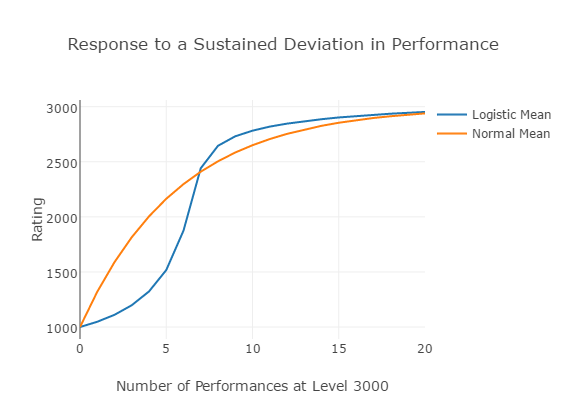
\includegraphics[scale=0.5]{../images/ResponsePlot.png} \end{center}

Had we tried to perform outlier reduction in a memoryless fashion, we would continue to increase the rating by 48 per match, oblivious to the possibility that the player truly did experience a sudden improvement. In Elo-R, the outlier status of a performance is treated as tentative. If later matches support the hypothesis of having improved, the rating will increase by an additional 63 points, followed by over 100 points in each of the third and following matches, as plotted by the blue curve above.

After six consecutive matches with $p_i = 3000$, the rating is 1875 and very unstable (even though $\sigma_i$ is unchanged!). The system is no longer sure which to trust: the extensive history at level 1000, or the smaller number of recent matches at level 3000. Depending on what comes next, the player's rating can very quickly fall toward 1000 or rise toward 3000. However, note that in either case, the change will not overshoot, say to 5000, unless enough new evidence is accumulated at that level. As the $p_i=3000$ streak continues, the seventh match on the blue curve jumps by a whopping 566 points. As the player's rating converges to 3000, the old $p_i = 1000$ data acquires outlier status, thus speeding convergence.

In contrast, while a system such as Codeforces does not compute $p_i$ values in quite in the same way, we can obtain a good approximation by removing outlier reduction from Elo-R, effectively treating the performances to be averaged as normal instead of logistic measurements. This makes the system effectively memoryless, since it turns out that each match simply moves the rating about 16\% closer to the new $p_i$ value, independent of the history. With this change, we obtain the orange curve, which jumps a whopping 320 points at the very first performance. Indeed, there is no limit: if you could find players whose ratings are extremely high, and beat them even once, your rating would take arbitrarily large leaps.

Note that this is not quite true of TopCoder, which incorporates a hack that caps the maximum rating change: if TopCoder's update formula demands too large a change, the cap kicks in. In contrast, Elo-R's cap is a natural and smooth consequence of its update formula and is sensitive to whether a change is charting new territory, or merely confirming a plausible hypothesis. TopCoder does attempt to make the magnitude of its updates sensitive to the amount of fluctuation in a player's history, using a volatility measure, but this measure does not account for the direction of the changes, resulting in the non-monotonicity flaw mentioned above.

Notwithstanding arguments that a high rating ought to properly be earned over multiple matches rather than a single fluke, the other danger is that these observations also hold in reverse: one bad day on Codeforces can seriously damage one's rating and negate several rounds of steady progress. By using heavy-tailed logistic distributions everywhere, Elo-R understands that unusually high or low performances do occasionally occur, and one round in isolation is never a reliable signal.

Interestingly, despite the slow start, the blue curve ultimately converges faster than the orange one. Since Elo-R uses its memory to dynamically adapt its view of potential outliers, it overtakes the orange curve as soon as new evidence outweighs the old hypothesis!

\subsection{Numerical analysis}

The ratings accumulate $O(\epsilon)$ numerical error per match, and likely a lot less in the long run due to statistical averaging...